\documentclass{article}
\usepackage{graphicx}  % Include the graphicx package
\usepackage{ifxetex,ifluatex}
\usepackage{bookmark}
\usepackage{cite}
\usepackage{adjustbox}
\usepackage{amsmath}
\usepackage{hyperref}
\usepackage{graphicx}
\usepackage{subcaption}
\usepackage{float}
\usepackage[a4paper, top=3cm, bottom=3cm, left=3cm, right=3cm]{geometry}

\begin{document}

\title{
  \vspace{-3cm}  % Adjust vertical space before the images
  \begin{minipage}{0.48\textwidth}
     \raggedright  % Aligne at the left
    
\includegraphics[width=0.6\textwidth]{images.png}  % First image on the left
   \vspace{2cm}
  \end{minipage}
  \begin{minipage}{0.48\textwidth}
    \raggedleft
 
    
\includegraphics[width=0.6\textwidth]{lepmi_logo.png}
    \vspace{2cm}
    % Second image on the right
  \end{minipage}
  \vspace{2cm}

  \textbf{\Large Influence of KCl and NaCl Proportions in\\
  ${Li(Ni}_{0.8}{Co}_{0.1}{Mn}_{0.1}{)O}_{2}$ \\ 
  \vspace{0.3cm}
  \textbf{\Large Molten Salt Synthesis for Li-ion Batteries}
    \vspace{4cm}
  }
 

\author{
  \textbf{Authors}\\
  Noriega Franco Santiago \\
  Choppe Apolline \\
  Brétillon Laura\\
  \\
  \textbf{Supervisors}\\
  Eddy Coron\\
  Julia Levy\\
  Lenka Svecova}


\date{
  \vspace{2cm}
  \small{January 24, 2024}
}




\maketitle
\newpage
\setcounter{page}{1}  % Start counting from 1
\tableofcontents

\listoffigures

\listoftables

\section{Abstract}
\section {Introduction}

\subsection{Context}

Lithium-ion batteries are a key technological tool for the sustainable mobility development all around the world. The performance of these batteries are highly influenced by the materials composition, morphology, crystal structure and synthesis parameters, specially for the positive electrode material and the electrolyte.\cite{topo} \\

NMC (Nickel-Manganese-Cobalt oxide) is todays the predominant material used for the positive electrode in modern electric vehicle batteries. Current developments focus on reducing cobalt content in favor of increasing nickel in the structure, specifically transitioning towards high-nickel compositions such as NMC811. This shift aims to enhance energy density, lower material costs, and address ethical and environmental concerns associated with cobalt mining. \cite{NMC811} \cite{NMCintro} \\

The specific theoretical capacity calculated with Faraday law:

\begin{equation}
Q_{th} = \frac{n F}{3.6 M} 
\end{equation}

where n: number of electrons;
Faraday constant F = 96500 C/mol;
M=96.5 mol/g mass molar of NMC811;

\begin{center}
  

\begin{tabular}{|c|c|c|}
  
  \hline
  Specific capacity
theoretical
(mAh/g) & 280  \\
  \hline
  Average Voltage in discharge (V) & 3.7  \\
  \hline
\end{tabular}
\end{center}

However, the higher nickel content introduces significant challenges. Nickel's tendency to occupy lithium sites, a phenomenon known as cation mixing or positive electrode mixing, can degrade the crystal structure. This defect reduces lithium mobility, diminishes cycling stability, and impairs the battery's long-term performance. Furthermore, high-nickel NMC materials are more chemically reactive, which can lead to thermal instability and increased side reactions with the electrolyte.\cite{NMCintro} \\

Currently, there is a great need to avoid any waste form industry,
specially if you are working with scarce materials. The European Critical Raw Materials Act describes lithium, nickel and cobalt as crucial for the economy and asks for the implementation of a sustainable independent supply chain.\cite{RMA} Therefore some efforts
have been done to repurpose the waste of Li-ion batteries plants and turn them into a usable material. This project, attached to LEPMI laboratory and VERKOR, aims to repurpose byproduct carbonates (\({MnCO}_{3}\), \({CoCO}_{3}\) and \({NiOH}_{a}{({CO}_{3})}_{b}\) ) for the synthesis of NMC811 using a molten salt-assisted solid-state sintering method. \\


\subsection{Close-up on the Molten Salts Method}
A prior study by the Karlsruhe Institute of Technology  worked on methods to 
synthesis of LNO using molten salts as a diffusive medium.
The aim of this study was to create a model for single crystal
layered lithium metal oxides (NCM's).\\
Here the molten salts as a tool to produce a single crystal
at relatively low temperatures.
The selected salts were NaCl, KCl, CsCl and \(K_{2}SO_{4}\), 
done at molar ratios to nickel from 1.0 to 4.0 \cite{meltingp}.\\
The results by SEM and XRD methods showed that the molar ratio
of the salts significantly affected the martials particle size with 
higher salt ratios, yielding in larger particles but not a special effect on the particle size distribution.
 The salt selection also affected the purity of the final sample \cite{meltingp}.

\subsubsection{A Less Energy-Intensive Method}
Traditional synthesis methods for NMC require temperatures exceeding 900°C, resulting in high energy consumption. One alternative to this is the introduction of a liquid diffusion medium into the process. The presence of a liquid phase during calcination accelerates the overall reaction kinetics, acting as a more efficient medium for particle growth and homogenization. Once the process is completed and the material has solidified, the liquid phase is no longer needed, as it could interfere with the purity of the target material. For this reason, molten salts are used. These salts can easily dissolve in water, allowing them to be washed away, ensuring the purity of the synthesized material after processing.\cite{Heuristics}

\subsubsection{Choice of Salts}
The requirements for the salt selection were the following:
\begin {itemize}
\item Low melting point: The salt melting point needs to be adequate 
for the synthesis methodology and parameters. This also depends on the material
that is wanted to be synthesized.
\item Chemical inertness: The salt should not react with the other substances in the mixture. 
Another important consideration is that the solvated ions of the salt should not take lithium sites on 
the electrode's crystal structure.
\item Cost Effectiveness. The economic viability of the salt is also an important factor to consider.
specially if the process is wanted for industrial applications. 
\end{itemize}
A mixture of NaCl and KCl is chosen for this process, as the combination of both salts lowers their melting point. This allows for the formation of a purely liquid phase at the temperature required for synthesizing NMC. Additionally, these salts are abundant and not expensive. Their ions are  large enough to not substitute lithium ions in the crystal lattice of the material during the washing step. \cite{Heuristics} \\

\subsubsection{Single-crystal (SC) particles formation interest}

The \textbf{molten salt synthesis} method is a technique producing single-crystal particles, unlike the polycrystalline particles typically obtained through the solid-state method. Using molten salts, which act as a reactive medium at high temperatures. In their liquid state, these salts provide an environment that enables free ion movement, facilitating controlled crystal growth. This process allows the formation of single-crystal particles by favorating uniform growth and minimizing the formation of grain boundaries that are characteristic of polycrystalline structures.

This phenomenon is more precisely known as \textbf{Ostwald ripening}, which plays a crucial role in the formation and growth of particles. When a mixture of particles of varying sizes is heated in the molten salts, smaller particles, which are thermodynamically less stable due to their higher surface energy, tend to dissolve. The ions released from these smaller particles migrate through the molten salt medium and redeposit onto larger particles, which are more stable because of their lower specific surface area. This process, enhanced by the high ionic mobility in molten salts, leads to a reduction in particle size dispersion and a gradual increase in average particle size. Over time, the smaller particles disappear entirely, leaving only the larger ones, which develop into well-defined single crystals.

Controlling the salt temperature and heating duration is crucial for tuning the final particle size. Higher temperatures and longer heating times accelerate the ripening process, resulting in larger particles. This precise control makes the molten salt method particularly advantageous to control size and morphology particles. \\


The focus of this study is to synthesize using this method as well as to evaluate how different proportions of NaCl and KCl in the salt mixture affect the final product (morphology, composition, purety) and to analyze the electrochemical performance of the NMC positive electrode material.\cite{meltingp}The morphology and performance of NMC 811 for lithium-ion technologies will be analyzed using characterization techniques: Scanning Electron Microscopy (SEM), X-Ray Diffraction spectroscpoy to identify the material phases as well as electrochemical characterization techniques on coin cells: Charge/discharge protocol.

\section{State of Art}

\subsection{Positive electrode materials}

Todays positive electrodes are mostly intercalation or composite electrodes, they consist in a solid network that can host lithium ions with intercalation during discharge and deintercalation during discharge.
These compounds can be devided into several different structures; layered, olivine and spinel. \cite{topo} \\

Some common cathode materials in lithium-ions technologies are:
\begin{description}
 \subsubsection{Layered structures}
  \item[$\text{LiCoO}_{2}$]  (LCO). This material has low capacity compared to the theoretical one the extraction of more than half the lithium content leads to structural instabilities. It's use is also restricted due to the high cost of cobalt and its scarcity. \cite{topo}\cite{LCO}
 
  \item[$ \text{Li(Ni}_{0.8}\text{Co}_{0.1}\text{Mn}_{0.1}\text{)O}_{2} $]  (NMC811). NMC811 has more nickel and less cobalt than NMC111, which is better for the environment by reducing reliance on cobalt. However, this higher nickel content makes NMC811 batteries less stable and more prone to degradation and overheating compared to NMC111.\cite{topo}
  

  \item[$\text{LiNi}_{0.8}\text{Co}_{0.15}\text{Al}_{0.05}\text{O}_{2}$] (NCA).
  This material increases the charge capacity by changing the Co content with Ni and using aluminum as 
  a stabilizer. This reduces slightly the average cell voltage
  compared to LCO.\cite{topo}
\end{description}

\begin{description}
 \subsubsection{Spinel structures}
  \item[$\text{LiMn}_{2}\text{O}_{4}$](LMO).The specific lattice structure
  of LMO, allows diffusion on three dimensions, which leads to faster charge
  - discharge rates. It is also a greener solution compared to to 
  Co based positive electrode materials. The disadvantage of LMO is t
its low charge retention and low cyclability.\cite{topo}
\end{description}

\begin{description}
  \subsubsection{Olivine structures}
  \item[$\text{LiFePO}_{4}$](LFP). This is also a greener material than the 
  Co based structures. LFP has a really high thermal stability but only counts
  with one dimensional diffusion. Therefore the voltage of discharge
  is too low.\cite{Olivine} \\
\end{description}

\subsection{Synthesis methods}

The choice of synthesis method plays a critical role in determining the final properties of NMC materials. Key attributes such as tap density, particle size distribution, particle morphology (both primary and secondary shapes), and crystallinity are strongly influenced by the synthesis process. Additionally, the method chosen impacts the presence of impurities, the overall quality of the final product, and its electrochemical performance. \\

Various synthesis methods are available for producing NMC, including co-precipitation, solid-state reaction, sol-gel processes, hydrothermal methods, and spray pyrolysis \cite{process}. 

Each approach has its own advantages and limitations, influencing the structure and performance of the material in different ways. Below is an overview of the most commonly used methods for NMC synthesis:
\subsubsection{Co-precipitation}
This is today the most popular and cost effective production method, on an industrial scale
. The method consists on the simultaneous precipitation of the transition metals and a subsequent sintering with
a lithium source. The parameters important for this process is the pH of the solution, the stirring rate 
and the used chealing agent this highly affects the particle size and morphology. \cite{process}  \\
There are three types of co-precipitation depending on the precursors used;
\begin{itemize}
  \item Carbonate co-precipitation: This type of precipitation doesn't need an inert atmosphere
  because the oxidation state of the metals can be stabilized by CO. The problem is that
the control of the final morphology is limited. \cite{process}
  \item Hydroxide co-precipitation: The final product of this process is really
  cost effective and has high tap density. When sintered, the particle size doesn't change
  so much but it is possible to get impurities from manganese oxides.\cite{process}
  \item Oxalate co-precipitation: This method is considered more environmentally
  friendly than the other two, and even cheaper. It does not require an inert 
  atmosphere. The only problem is that the oxalate salts that are used 
  have low solubility in water, therefore the production rate would be lower\cite{process}.
\end{itemize}

\subsubsection{Sol-gel}
Sol-gel method is used on laboratory scale conditions. It consists on forming a gel from transition 
metal salts and a chealing agent that is then dried and sintered. It provides really good morphology and control over the stoichiometry\cite{process}.

\subsubsection{Solid state reaction}
This is one of the most classical methods to synthesize any kind of ceramic material. 
It consists on the correct mixing of the precursors, and then heating the powder below the fusion temperature of the material.
This activates the diffusion of the material due to surface energy phenomena, finishing on the coarsening of larger particles
in expense of smaller ones. The disadvantage of this method is the high dependence on the initial particle size distribution and 
the homogeneity of the mixture\cite{process}.

\subsubsection{Spray pyrolysis}
Spray Pyrolysis consists on atomizing the precursor in a solution at a really high temperature. This yields on a 
quite homogenous layer of mixed materials (not better that CVD or PVD). Here the properties depend on the solution concentration, the 
droplet size and the temperature of the process\cite{process}.

\subsection{Characterization methods}
There are several techniques to extract information from positive electrode materials,
these evaluate physical, chemical and electrochemical properties to evaluate the stability, morphology 
and performance of the material. Here is an overview of the characterization techniques used on this project.\\
\subsubsection{Scanning Electron Microscopy (SEM)}
This technique is useful to get high resolution imaging of the materials morphology.
It consists on a beam of electrons that scans the surface of the sample and the collection of three 
different signals; secondary electrons, backscattered electrons and X-rays. With the primary electrons 
being the ones emitted by the source.\\
\begin {itemize}
\item Backscattered electrons: These electrons are the ones that interact with the materials atoms and get back to
the sensor, the intensity of the signal can be related to the element's atomic mass. Heavier elements will scatter more electrons
to the sensor. Therefore, this signal is useful to get the composition and phases of the material.
The strength of this signal is also dependant on the topography of the samples surface, therefore a topographic image can be obtained.\\
\item Secondary electrons: The secondary electrons are the ones that interact in an inelastic way with the material, therefore they arrive to
the sensor with less energy. This signal is useful to get the morphology of the material because only the electrons that interact with the surface
are collected. The energy when collected is related to the surface morphology and an image is created.\\
\item X-rays: Are a byproduct generated when a primary electron removes an electron from the inner shell of an atom. The energy of the X-ray is related to the
atomic number of the element. This signal is useful for the creation of composition maps overlaying the 
SEM images.\\
\end{itemize}

\subsubsection{X-Ray Diffraction (XRD)}
X-Ray Diffraction is a non destructive technique used to characterize crystalline materials. 
It provides information about the crystal phases, structural parameters (ize of crystals, crystallinity  and defects) and the orientation of the crystals.\\
This method works by comparing the of the xray beam (with a wavelength $\lambda$) and the lattice planes called $\theta$. The reflected beam has an angle of $2\theta$, and this is the one that is measured.


\begin{equation}
2d \sin(\theta) = n\lambda   
\end{equation}

The Bragg's law is used to calculate the distance between the lattice planes (d), characteristic of the crystal structure. 
The intensity of the diffracted beam is related to the number of atoms in the crystal, the atomic number and the distance between the planes.\\

Today, databases can compare the diffraction spectra with the ones of known materials, to identify the phases present in the sample.\\

\subsubsection{Electrochemical characterization}
 
\section {Methodology} 
\subsection{NMC 811 electrode synthesis}

\subsubsection{Active material synthesis}

\textbf{Step 1: precursor mixing: }\\
Precursor mixtures were prepared with the stoichiometry of NMC811
 with excess lithium 15\%, and with the target of 4g of precursors. As three salt ratios are tested, three NMC precursors need to be made. Each species was weighted as stated in Table \ref{t1} in the three samples, and the salts were then added with different mass for each mixture according to Table \ref{t2}.
\begin{table}[h!]
    \centering
    \begin{tabular}{|c|c|}
        \hline
        \textbf{Species} & \textbf{Mass (g)} \\ 
        \hline
        MnCO$_3$ & 0.589 \\
        CoCO$_3$ & 0.610 \\
        Ni(OH)$_a$(CO$_3$)$_b$ & 4.508 \\
        LiOH & 2.828 \\
        \hline
    \end{tabular}
    \caption{Mass of each components used for NMC 811 synthesis other than the salts.}
    \label{t1}
    
\end{table}
\begin{table}[h!]
  \centering
  \begin{tabular}{|c|c|c|c|}
    \hline
    \textbf{Salt ratio (NaCl:KCl)} & \textbf{Mass of NaCl (g)} & \textbf{Mass of KCl (g)} & \textbf{Total mass (g)} \\ 
    \hline
    1:1 & 2.971 & 3.791 & 6.762 \\ 
    6:4 & 3.566 & 3.033 & 6.598 \\ 
    4:6 & 2.377 & 4.549 & 6.926 \\ 
    \hline
  \end{tabular}
  \caption{Masses of NaCl and KCl for different salt ratios used in NMC synthesis.}
  \label{t2}
\end{table}


\textbf{Step 2: Ball milling:}\\
Each sample is then mixed with ball milling, using 60 ZrO2 4.5mm beads in a 45 mL bowl air and 4 cycles of the following programme: rotations at 250 rpm during 5 min, then 10 min rest. \\

\textbf{Step 3: Pre-annealing:}\\
The three mixtures obtained are then heated at 500°C in an oven: first, a ramp of 5°C/min during 100 min to reach 500°C, then this temperature is held during 3h. This step aims to melt the LiOH in the precursors, as this Li-source melting point is 462°C. \cite{precalci} \\

\textbf{Step 4: Annealing:}\\
The pre-annealed samples are then calcinated in an oven at 800°C for 12h, after a ramp of ??. The salt mix melts, as its melting point is at 660°C, but not the NMC material as it melts above 800°C. When the samples are annealed, they are then cooled down naturally.\\

\textbf{Step 5: With or without ball milling:}\\
Each annealed NMC precursor are grounded in a morter and divided in two samples: an  A one and a B one, that will follow different protocols. The samples B have a additionnal ball milling step, with the same parameters as before: 4 cycles of rotations at 250 rpm during 5 min cut by 10 min rest, using 60 ZrO2 4.5mm beads in a 45 mL bowl air. The goal is to homogenize the grains again. As for samples A, they are not ball milled and go directly to the next step of the protocol.\\

\textbf{Step 6: Washing:}\\
Each one of the grounded or ball-milled NMC samples are then washed using vacuum filtration. The filters used are 47 mm Milipore Express PLUS 0.22µm PES Membrane, and the powder is added on top. It is rinced several times with distilled water to remove the salt from the NMC material, with approximately 250 mL of water in total. NaCl and KCl then dissolve in the water as  $Na^+, K^+$ and $ Cl^-$ and pass through the filter, leaving the NMC powder. The solid material is dried in the air after the washing, to remove the water. \\

\textbf{Step 7: Last annealing:}\\
After the washing step, the samples are once again heated in the oven, this time at 600°C for 3h with a prior ramp of ??. This last step of the NMC 811 materials synthesis aims to release the CO2 gas that can still remains in the powder, or even some carbonates. It is also a way to effectively dry the material previously washed.\\

\subsubsection{Ink preparation}
To make a functioning positive electrode to be tested inside a coin cell, 
the NMC 811 obtained needs to be mixed with a conductive carbon and a binder into a slurry.
This mixture needs to be composed by 80\% of NMC 811 (active material), 10\% of carbon black (CB) and 10\% of binder (PVDF).\\

Here, the carbon black is used as a conductive matrix, and helps create ionic paths for the electrolyte to fill the pores and have a good contact with the NMC 811\cite{Itou}. The binder is a polymer called polyvinylidene difluoride (PVDF),
is used to keep the material together.\\

NMP (N-Methyl-2-pyrrolidone) is used as the solvent to adjust the viscosity of the ink. It should be added gradually to avoid clumps. Cyclohexane can be added to improve dispersion of active material in the mixture, it evaporates quickly under the hood when heated to 80°C.\\

\textbf{Process of Ink Preparation:}\\
\begin{itemize}
  \item The NMC, carbon black and PVDF are weighted in the correct proportions that are represented on 
  table \ref{t3}.
  \item The materials are first mixed in a speed mixer (Hauschild SpeedMixer DAC 250.3 SP)  at 1500 rpm for 2 minutes to ensure all particles are coated. A second mixing step at 2500 rpm for 8 minutes, with additional NMP, is performed to achieve the desired consistency.
  \item The ink is then coated onto aluminum foil using an adjusted blade of 15 um. Proper ventilation must be ensured during the process, and the blade used for coating should be cleaned beforehand. Coating is performed at a low speed for uniform application. The desired wet thickness is 150 µm, which dries to 20-30 µm, when applied on aluminum.
  \item The electrode coating was dried in an oven for 12 hours, after which it was cut using a punch cutter. Three electrodes, each with a diameter of 12 mm, were then weighed to ensure consistent weight across samples, thereby maintaining the same active material mass.
  \begin{itemize}
    \item The NMC, carbon black and PVDF are weighted in the correct proportions that are represented on 
    table \ref{t3}.
    \item The materials are first mixed in a speed mixer (Hauschild SpeedMixer DAC 250.3 SP)  at 1500 rpm for 2 minutes to ensure all particles are coated. A second mixing step at 2500 rpm for 8 minutes, with additional NMP, is performed to achieve the desired consistency.
    \item The ink is then coated onto aluminum foil using an adjusted blade of 15 um. Proper ventilation must be ensured during the process, and the blade used for coating should be cleaned beforehand. Coating is performed at a low speed for uniform application. The desired wet thickness is 150 µm, which dries to 20-30 µm, when applied on aluminum.
    \item The electrode coating was dried in an oven for 12 hours, after which it was cut using a punch cutter. Three electrodes, each with a diameter of 12 mm, were then weighed to ensure consistent weight across samples, thereby maintaining the same active material mass.
\end{itemize}

The active material mass (mg) was calculated as:

\begin{equation}
m_{\text{active}} \, (\text{mg}) = 0.8 \times m_{\text{total}} \, \quad \text{(for NMC811)}
\end{equation}

\item The thickness of the coating was measured using a thickness gauge. This measurement was used to calculate the coating volume and subsequently the porosity:

\begin{equation}
\text{Porosity} (\%) = 100 \cdot \left( 1 - \frac{\text{Coating Volume}}{\text{Theoretical Volume}} \right)
\end{equation}

Where the  coating volume is the thickness times the area of the electrode. 
  
\begin{table}[h!]
  \centering
  \begin{adjustbox}{width=1\textwidth}
  \small
  \begin{tabular}{|c|c|c|c|c|c|}
    \hline
    & \textbf{Total Mass (mg)} & \textbf{Active material mass (mg)} & \textbf{Theoretical volume (mm$^3$)} & \textbf{Porosity (\%)} & \textbf{Theoretical capacity (Ah)} \\ 
    \hline
    \textbf{Na 6:4 K} & 4.20 & 3.36 & 1.19 & 52.06 & 3.3 \\ 
    \hline
    \textbf{Na 4:6 K} & 4.80 & 3.84 & 1.36 & 51.79 & 3.8 \\ 
    \hline
    \textbf{Na 1:1 K} & 5.30 & 4.24 & 1.51 & 52.47 & 4.2 \\ 
    \hline
  \end{tabular}
  \end{adjustbox}
  \caption{Parameters for electrode tape casting.}
  \label{t3}
\end{table}
\subsection{Coin cell protocol}

\subsection{Characterization precaution}


\section{Results and discussion}

\subsection{Morphology and composition analysis}
\subsubsection{Homogeneity of the NMC material}
\subsubsection{Size and shape analysis}
\subsubsection{XRD analysis: phase analysis}
%\subsubsection{Lithium amount in  ${Li}_{x}(Ni}_{0.8}{Co}_{0.1}{Mn}_{0.1}{)O}_{2}$ }

\begin{figure}[H]
    \centering
    % Ligne 1 : Première sous-figure avec deux images côte à côte
    \begin{subfigure}[t]{0.45\textwidth}
        \centering
        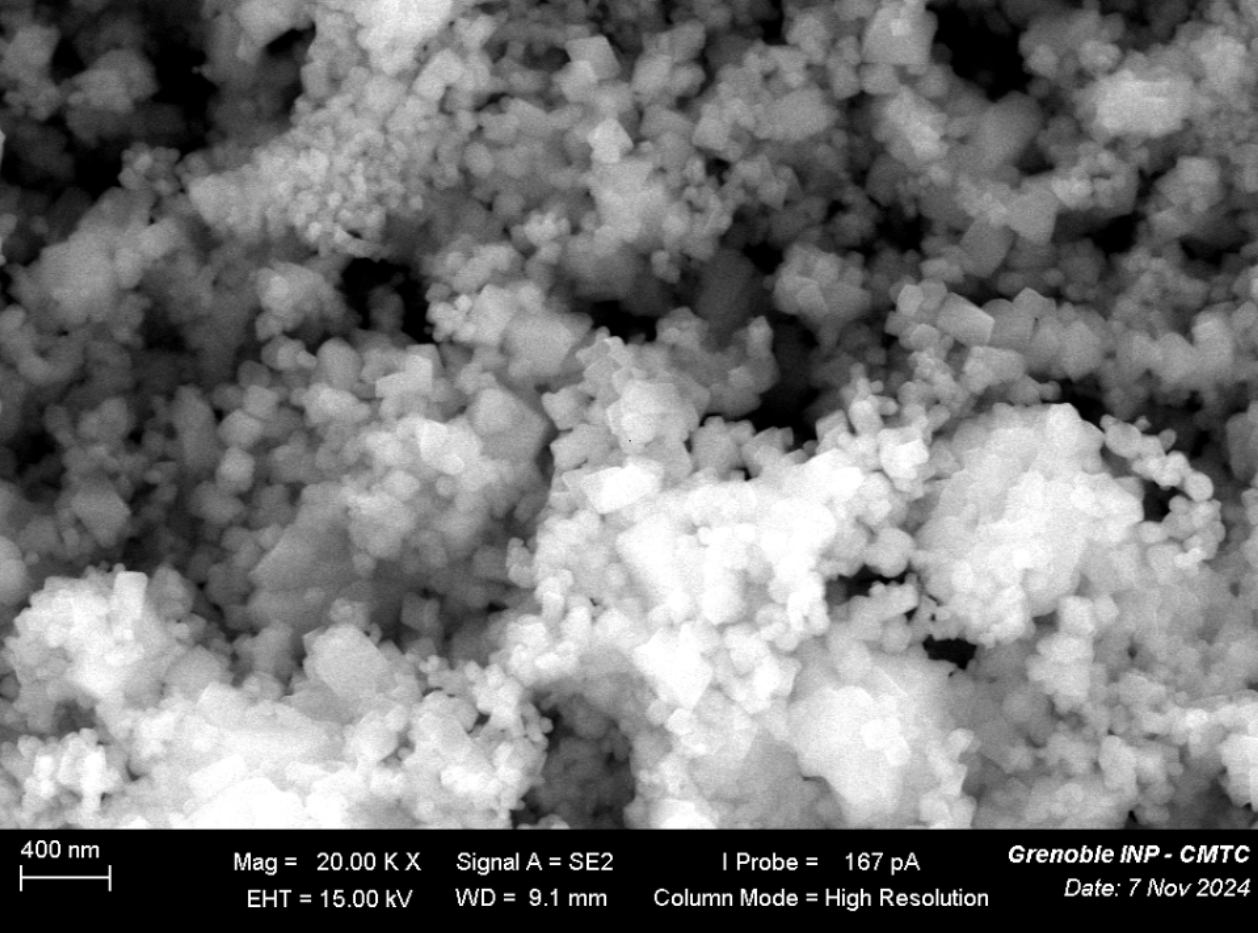
\includegraphics[width=\textwidth]{NMC_11_legend.png}
        \caption{NMC 11 }
    \end{subfigure}
    \hfill
    \begin{subfigure}[t]{0.45\textwidth}
        \centering
        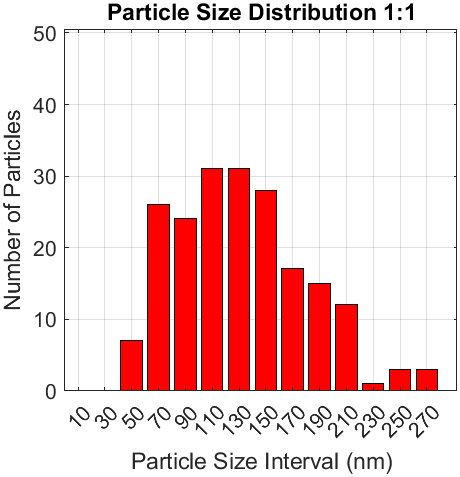
\includegraphics[width=\textwidth]{NMC11SEMDIST.png}
        \caption{}
    \end{subfigure}

    \label{fig:SEM_Distributions}
\end{figure}

\subsection{Understanding the steps of NMC synthesis}


\section{Conclusion}


\bibliographystyle{plain}  
\bibliography{Biblio}

\section{Annexes} 
\begin{figure}[H]
  \centering
  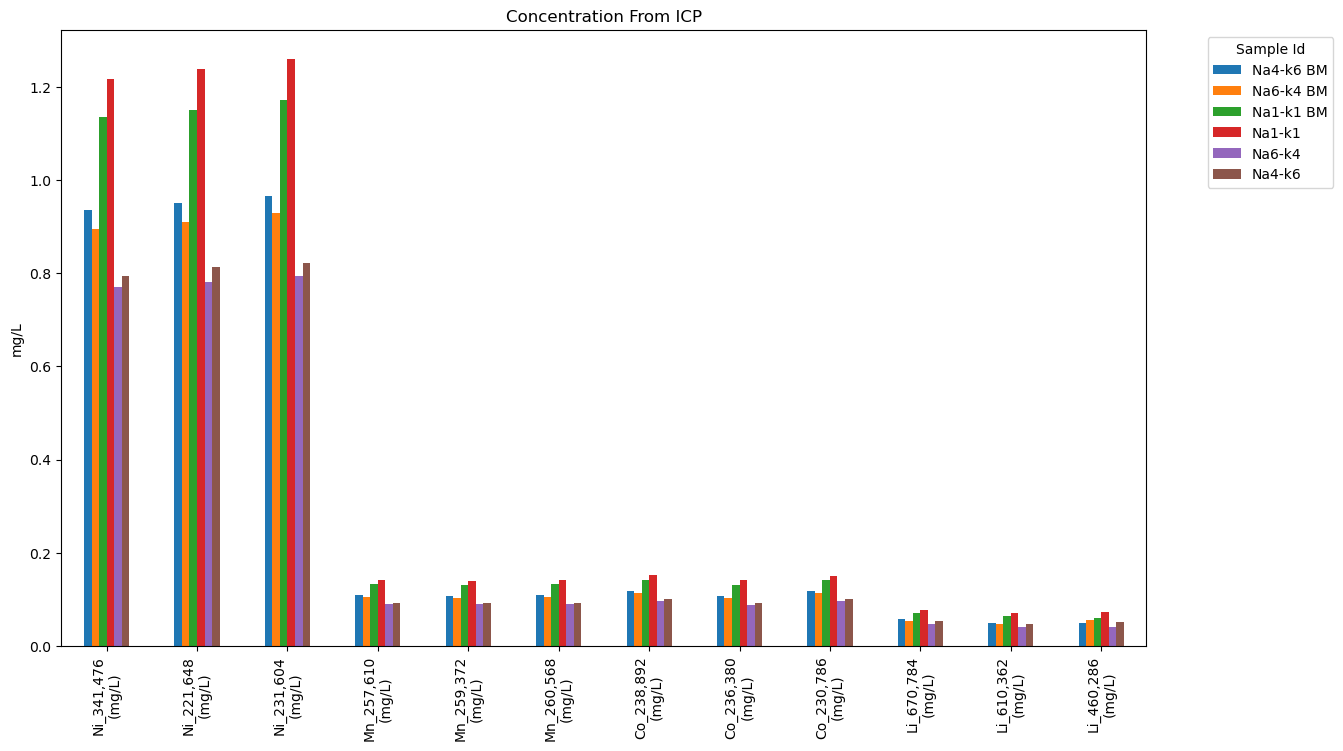
\includegraphics[width=\textwidth]{output.png}
  \caption{ICP readings direct results for every sample.}
  \label{fig:example_image}
\end{figure}
\begin{figure}[H]
  \centering
  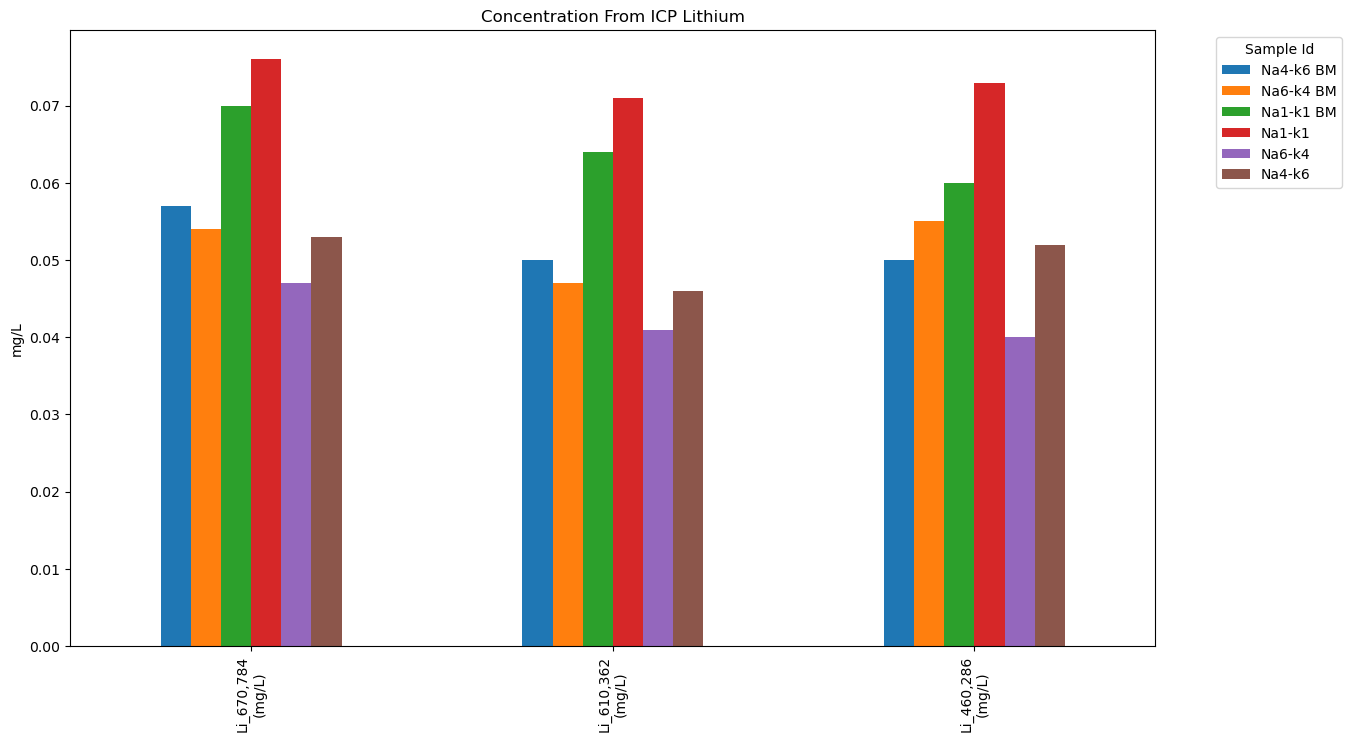
\includegraphics[width=\textwidth]{output3.png}
  \caption{Lithium specific ICP readings direct result.}
  \label{fig:example_image}
\end{figure}
\begin{figure}[H]
  \centering
  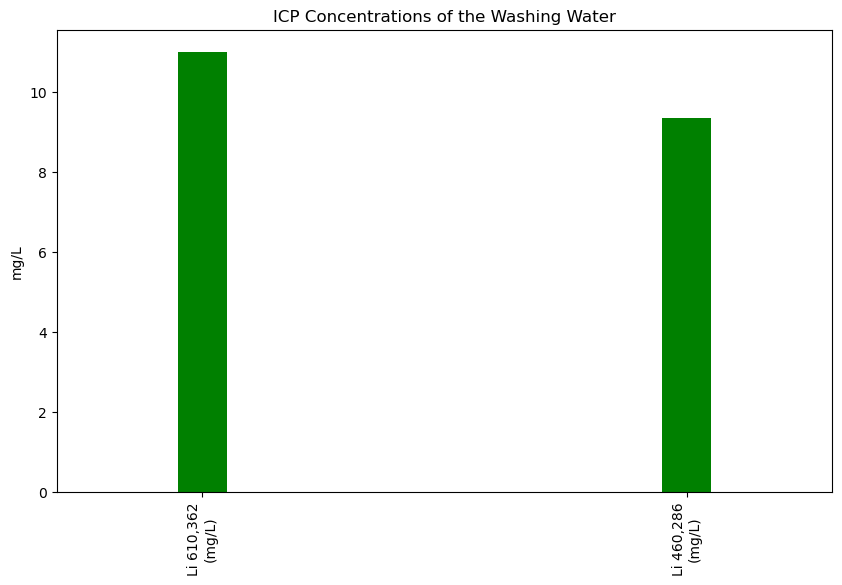
\includegraphics[width=0.8\textwidth]{output2.png}
  \caption{ICP readings for the washing water }
  \label{fig:example_image}
\end{figure}

\end{document}


